\documentclass[12pt]{article}
\title{\textbf{Perceptions \& Use of BitTorrent P2P File Sharing by Dartmouth College Students\footnote{This paper constitutes the final project for the Fall 2013 iteration of CS 55: Security and Privacy, taught by Charles C. Palmer, Adjunct Professor of Computer Science, Dartmouth College; CTO Security and Privacy, IBM Research.}}}
\author{
	Alex Gerstein \\ Dartmouth College\\ Computer Science, Film Studies\\ \texttt{alex.gerstein@dartmouth.edu} 
	\\ \\
	Scott Gladstone \\ Dartmouth College\\ Computer Science, Economics\\ \texttt{scott.gladstone@dartmouth.edu}
	}
\date{\today}

\usepackage[margin=1.0in]{geometry}
\setlength{\parskip}{10pt plus 1pt minus 1pt}
\usepackage{fancyhdr}
\usepackage{enumerate}
\usepackage{multicol}
\usepackage{fixltx2e}
\usepackage{graphicx}
\usepackage[font=small,labelfont=bf]{caption}
\usepackage[superscript,biblabel]{cite}

\begin{document}

\maketitle
\begin{abstract}
In our final project, we hope to investigate peer-to-peer (P2P) file sharing network protocols, specifically those related to torrenting (BitTorrent). After a general overview of the system and security flaws present, we plan to examine P2P in the context of Dartmouth College. By surveying students and speaking to Dartmouth College Computing Services, we hope to understand the disparity between the perception and actual use by students of torrent networks. If available, we also hope to obtain and analyze data from the College on student bandwidth habits, download frequencies, or other metrics that the College records. The outline below summarizes the questions we hope to answer and the individuals we hope to speak with.
\end{abstract}

%%%%%%%%%%%%%%%%%%%%%%%%%%%%%%%%%%%
%%%% ********			INTRODUCTION  		******** %%%%%
%%%%%%%%%%%%%%%%%%%%%%%%%%%%%%%%%%%

\pagebreak
\section{Introduction}

BitTorrent is a protocol supporting peer-to-peer (P2P) file sharing that facilitates the distribution of large data files over the Internet \cite{BitTorrent}. BitTorrent is one of the most common protocols for transferring large files and is often used for distribution of very popular files and files available for free, such as literary texts, audio files, movies, and applications. ``Torrenting'' is the process by which a user engages with a BitTorrent client in order to send and receive those desired files. To understand the uniqueness -- and security implications -- of the BitTorrent protocol, one must first develop a working understanding of P2P file sharing. From there, the legal implications of P2P file sharing and BitTorrent can be made clear. With this foundation, the authors then describe a study in which data about student perceptions of torrenting at Dartmouth College are compared with data collected by Dartmouth College network administrators describing student incidences of torrenting. Conclusion and policy recommendations are then made with the goal of aligning student perceptions and administrative desires.

\subsection{Peer-to-Peer (P2P) File Sharing}
According to one Internet dictionary, P2P is a ``type of Internet network that allows users with the same program to connect with each other and access files on one another's hard drives without the intervention of a server computer,'' \cite{NYTimes}. This decentralized network architecture consists of individual nodes called \emph{peers} that act as both suppliers and consumers of resources. In P2P networks, tasks are shared among multiple, interconnected peers who each make a portion of their resources -- processing power, disk storage, or network bandwidth -- available to all network participants, without the centralized coordination of a server-client model \cite{scholl}. A comparison of a decentralized-P2P network and a centralized server-based network are presented in Figure 1 and Figure 2 below.

\begin{figure}[h!]
\centering
\begin{minipage}[b]{0.45\linewidth}
	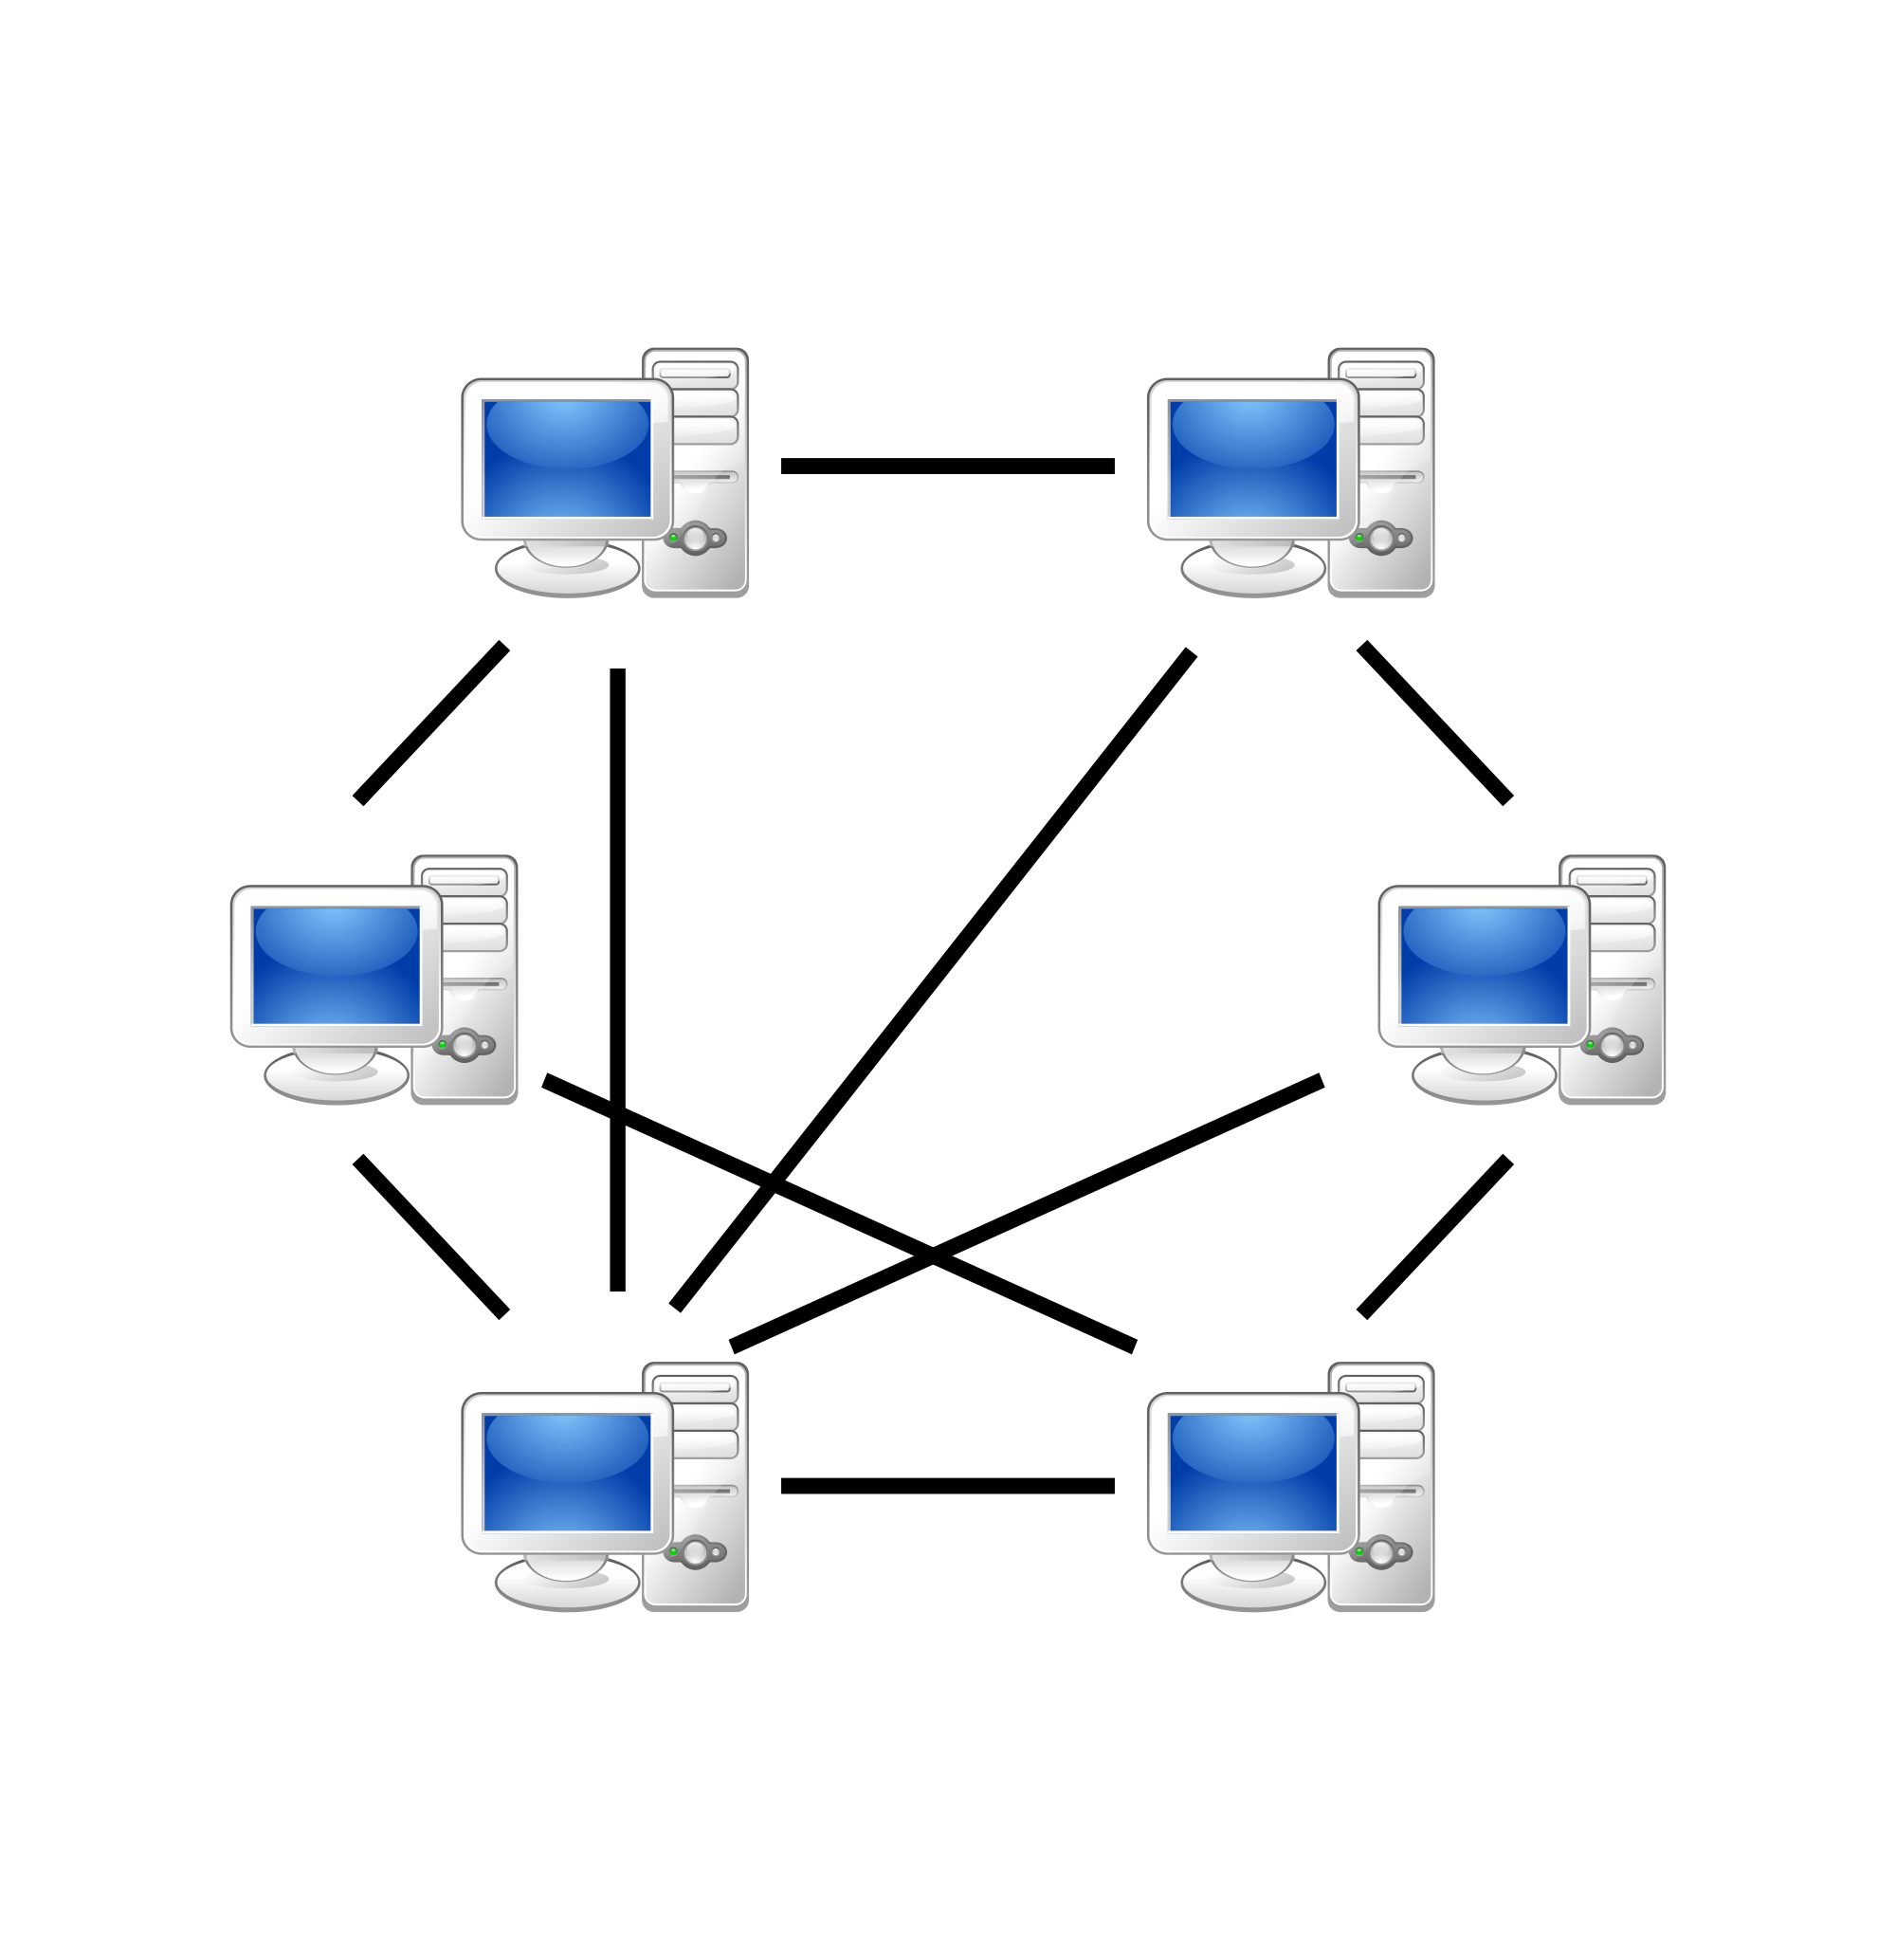
\includegraphics[width=56mm]{P2P-network}
	\caption{A peer-to-peer (P2P) network with interconnected nodes (``peers'') sharing resources. Source: Wikipedia.}
	\label{p2p_network}
\end{minipage}
\quad
\centering
\begin{minipage}[b]{0.45\linewidth}
	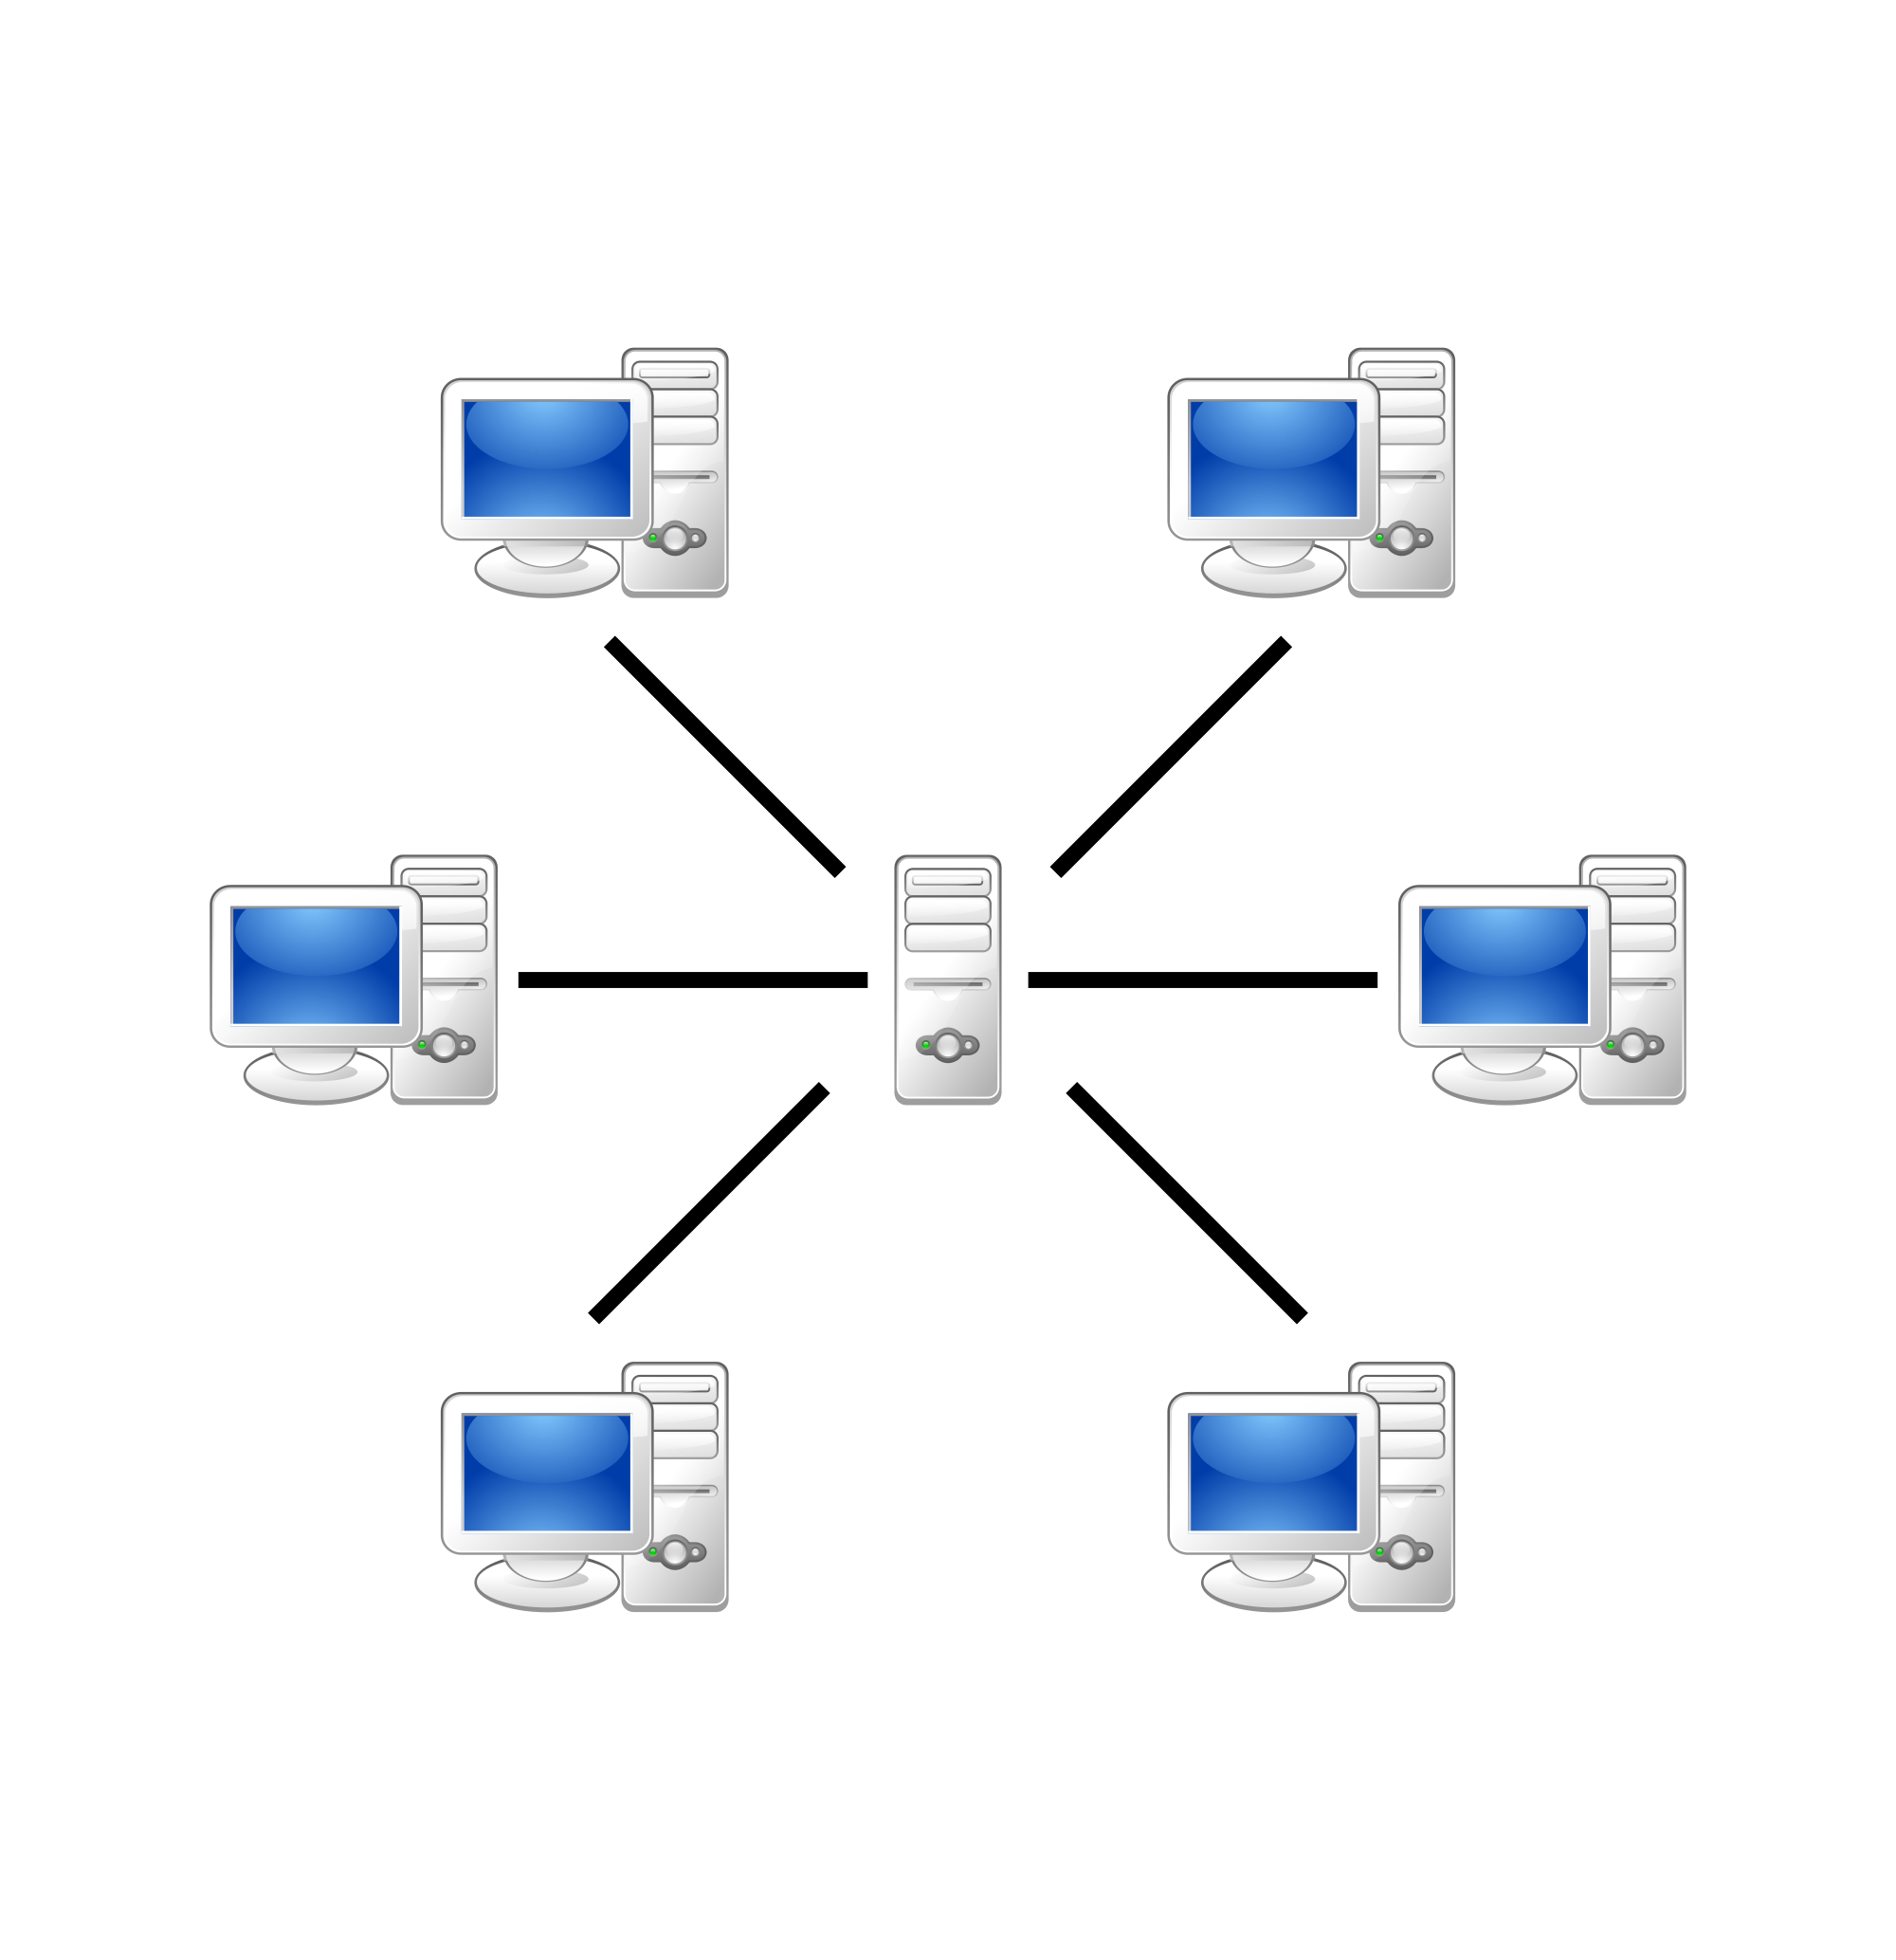
\includegraphics[width=56mm]{Server-based-network}
	\caption{A client-server model network, where individual clients request services from centralized servers. Source: Wikipedia.}
	\label{p2p_network}
\end{minipage}
\end{figure}

P2P networks are often found in residential home networks, allowing users to configure their computers in peer workgroups to allow sharing of files, printers, and other resources among all devices; with a number of computers running similar network protocols, P2P is a convenient way to access shared resources \cite{About}. However, the term ``P2P'' used today generally does not refer to the network architecture from which its name is derived, but to P2P file sharing systems. Using P2P software applications such as Napster or Kazaa, users are able to search for, transfer, and download data files over the Internet with any user on the same P2P file sharing network. The implications of such a system were huge: if \emph{any} user on the system had a file that another user demanded, the second user could -- via the network -- obtain the file. The second user would then also be a source of the file in the P2P network, making it faster and easier for more users to download the files. 

The first P2P file sharing networks, such as the purely-mp3 sharing network Napster, relied on a central index server to assist with the transfer of files. When someone searched for a file, the central index server -- which contained an index of all of the users and their shared content -- searched for all available copies of the file and presented them to the user; the file would then be transferred directly between the two private computers \cite{P2PFileSharewiki}. Because the file sharing occurred over a central network, Napster was held liable for copyright infringement over the sharing of mp3 files and was shut down in 2001 \cite{napster}. New protocols such as BitTorrent represent a technological evolution of P2P file sharing networks.

\subsection{BitTorrent Protocol}

BitTorrent is a P2P file sharing protocol that makes use of unique design to reduce the bandwidth and download time for more frequently requested data. The protocol allows a single user to download files quickly by allowing users to join a ``swarm'' of hosts to download and upload from each other simultaneously. Thus, instead of attempting to transfer a large file from one user to another like other P2P network protocols -- a slow, bandwidth-intensive process --, BitTorrent allows a user to download small segments of the file from a variety of users, significantly reducing computational energy and download time\cite{BitTorrent}. Because of this design, BitTorrent is often used for distribution of very large files, very popular files, and files available for free, as it is more efficient to distribute these files using BitTorrent than a regular download.

When a user ``torrents'' a file, meaning that the user is attempting to download a file over a P2P network using a BitTorrent client implementing the BitTorrent protocol, they begin by loading a .torrent file into a BitTorrent client. A .torrent file is a computer file that contains metadata about files to be distributed, including file names, sizes, checksums of all individual pieces, and a list of the network locations of ``trackers'' -- a server that facilitates communication between peers on a P2P network -- to help participants in the system seeking to download the same data find one another \cite{HTG}. The tracker shares the peers' IP addresses with other BitTorrent clients in the ``swarm,'' the group of all peers sharing a torrent. Each piece of a file specified in a torrent is protected by a cryptographic hash contained in the .torrent file; this ensures that any modification of the piece can be easily detected, preventing a user from downloading both accidental and malicious modifications of any pieces of a file \cite{BitTorrent}.

Once connected, a BitTorrent client downloads bits of the files specified in the torrent in small pieces, downloading different segments from data from different computers in the swarm. Once the BitTorrent client has some data, it can then begin to upload that data to other BitTorrent clients in the swarm; by using both downloading and uploading bandwidth and dividing the files into pieces, the time required to download the file is significantly reduces \cite{BitTorrent}. Thus, it is worth noting the following concept: ``Everyone downloading a torrent is also uploading the same torrent. If 10,000 people are downloading the same file, it doesn't put a lot of stress on a central server. Instead, each downloader contributes upload bandwidth to other downloaders, ensuring the torrent stays fast," \cite{HTG}. From this protocol, clients never actually download files from the tracker itself; the tracker keeps track of the clients connected in the swarm, but does not actually participate in the process of downloading or uploading data \cite{HTG}.

The process of sharing data via BitTorrent starts with a \emph{seed}, or the initial machine possession 100\% of the data. Then \emph{leechers}, also known as \emph{downloaders}, which refers to peers that do not have the entire file or are in the process of downloading the file. As the number of downloaders increases, the reliance of new leechers on old leechers decreases, as each successful downloader becomes a source of the file for future downloaders \cite{glossary}. From that point, the process repeats and continues, allowing peers on the network to share any and all files to which any other peer has access.

%\subsection{BitTorrent Security Concerns}
%What are security issues related to using BitTorrent? torrent poisoning (wiki)

%%%%%%%%%%%%%%%%%%%%%%%%%%%%%%%%%%%
%%%% ********			LEGAL ISSUES  		******** %%%%%
%%%%%%%%%%%%%%%%%%%%%%%%%%%%%%%%%%%

\section{Legal Issues \& Security Implications}

While the BitTorrent protocol itself is legal, those who use the service often do so to obtain files illegally. Illegally obtaining files, also known as digital piracy, involves sharing copyrighted media such as games, music, movies, TV shows, and software that the user does not have permission to share; whether the user is downloading or uploading content, involvement in this type of non-permitted operation is considered a violation of copyright law (http://www.ehow.com/info\_10004321\_define-illegal-downloading.html). In a 2010 sampling of the one thousand most actively seeded torrent files, 89 percent of the files were confirmed to be illegally shared and the majority of the remaining 11 percent were determined to be ``likely infringing,'' (http://arstechnica.com/tech-policy/2010/07/only-03-of-files-on-bit-torrent-confirmed-to-be-legal/). Only three files, or 0.3\%, were confirmed to be legal. The analysis of student's perception of torrenting will focus on the sharing of the illegal torrents, which comprise the overwhelming majority of the data shared through BitTorrent clients.

\subsection{Implications for Individuals and Network Hosts}

The entertainment industry and various anti-piracy groups have made numerous attempts to thwart those who torrent illegally. These methods, referred to collectively as torrent poisoning, are effective in both slowing download speeds and gathering IP addresses of the downloaders (http://en.wikipedia.org/wiki/Torrent\_poisoning). Organizations pose as seeders of a torrent to connect to leechers. Once this connection is made, the anti-piracy organization can save the user's IP address and deter the user from downloading or sharing the file. Counterpiracy companies, such as the now defunct MediaDefender, slow the download of files through numerous methods. These methods are mostly based on seeding or linking to fake files. For example, in a decoy insertion, seemingly uncorrupted versions of a file are distribute on a network to appear indistinguishable from the original files. While a decoy insertion targets the torrent files, a spoofing attack targets the locations of torrents to redirect potential leechers to non-existent locations. 

Both these attacks are founded on the principle that some downloaders will give up out of frustration. However, sometimes copyright enforcers take extreme measures to pro-actively prevent BitTorrenting. In 2007, Comcast was accused of hindering the uploading of complete files to BitTorrent. The following year, they were ordered to terminate their "unreasonable" network management. MediaDefender possibly overstepped their legal rights similarly in 2008 when they caused a Denial of Service attack on Revision3, a legal Internet television network distributor.

In the "real-world," the legality of torrenting and possible actions an external party can take against torrenters is a little fuzzy. However, when a college student signs an acceptable-use policy for the campus network, their rights become a little clearer, but only slightly.
	
\subsection{Dartmouth College Policy and Practice}
In Dartmouth College's "Acceptable Use Policy," users agree to not "post, use, or transmit content that you do not have the right to post or use; for example, [content] under intellectual property, confidentiality, privacy or other applicable laws" (http://www.dartmouth.edu/comp/about/policies/acceptable\_use\_policy.html). Furthermore, Dartmouth's "Copyright Policy \& Guidelines" includes the "copying and sharing images, music, movies, television shows or other copyrighted material through the use of P2P technology" as a probable violation of the "Copyright Law" (http://www.dartmouth.edu/copyright/peer2peer/index.html\#P2P)

Although the College does not police students' torrenting activities, it often receives formal legal notices from organizations like the Recording Industry Association of America (RIAA) or BayTSP (representer of movie and television studios) for infringers to discontinue their illegal activity. The College is required, by law, to forward these notices to the students responsible.

If a user continues his/her behavior after he/she is issued this warning, College Policy states that Dartmouth is permitted to revoke the user's access to its information technology resources. Additionally, any civil liability pushed by the anticopyright organizations%%%%%%%%%%%%%%%%%%%%%%%% UNFINISHED %%%%%%%

%%%%%%%%%%%%%%%%%%%%%%%%%%%%%%%%%%%
%%%% ********	     METHODS, DATA & ANALYSIS  	******** %%%%%
%%%%%%%%%%%%%%%%%%%%%%%%%%%%%%%%%%%

\section{Methods, Data \& Analysis}
The goals of this research were three-fold: first, to determine the student perception of the occurrence of torrenting at Dartmouth; second, to investigate the actual occurrence of torrenting at Dartmouth based on data provided by Dartmouth College Computing Services; and third, to examine the relationship between student perceptions and actual incidences of torrenting and make policy recommendations with the purpose of aligning student perceptions and student network activity. The methods employed to carry out these goals and the data collected are described in the sections 3.1 to 3.3.

\subsection{Student Perception Survey}
%Goals, Questions, and Distribution
\subsubsection{Participants}
The participants in the survey were 130 students at Dartmouth College. The population consisted of second-year, third-year, and fourth-year students at the College. Participation was anonymous and voluntary. All prospective participants were sent a link to a Google Form that was used to create the survey; all participants had completely voluntary choice in clicking on the link, examining the questions, and completing and submitting the survey. The population examined in this study may be biased in the sense that many individuals who completed the survey could have personally known the researchers or were members of CS 55: Security \& Privacy, the class for which this research was completed.

\subsubsection{Survey Design}
The survey was designed via Google Forms and was administered by providing a link to the survey to all prospective participants. The survey consisted of seven questions, six of which were mandatory. The mandatory questions asked the participant for his/her person experience with torrenting, whether they believed other students at Dartmouth torrented, the number of files that they believed the average student torrented, whether they believed Dartmouth recorded information about student torrenting, and whether their knowledge of Dartmouth Copyright Violation Policy impacted the amount that they torrented. The seventh, optional question asked whether the participant has any thoughts as to how Dartmouth College could reduce the incidence of torrenting on campus. All surveys were timestamped when submitted and resubmissions/changing of answers were not permitted. See Appendix A for a copy of the survey administered. 

\subsubsection{Perception Data}
Of the 130 students, 78 (60.0\%) stated that they had previously downloaded a file via torrenting in general, but only 52 (40.0\%) stated that they had downloaded files via torrenting while at Dartmouth. This indicates that 52 out of 78 individuals (74.3\%) who had torrented in general had also torrented while at Dartmouth. Of the 52 students who designated that they torrented at Dartmouth, 34 (65.4\%) claimed to download one to five files per month, on average; 5 (9.6\%) claimed to download zero files per month on average; 5 (9.6\%) claimed to download six to ten files per month on average; and 9 (17.3\%) claimed to download 11 or more files per month on average. 

Considering all students (both torrenters and non-torrenters), 82 of 130 students (63.1\%) claimed to download zero files per month on average. This was highly significantly different (\emph{p}$<$.00001) from the 16 (12.3\%) that those participants believed that the average Dartmouth downloaded via torrenting on average. The median self-reported number of files downloaded via torrenting on average was zero, while the median perceived number of files downloaded by the average student was one to five; based on the distributions presented in Figures 3 and 4 below, there is a clear right shift in Figure 4 as compared with Figure 3, indicating that there is a significantly higher perception of student torrenting than what actually occurs.

\begin{figure}[h!]
\centering
\begin{minipage}[b]{0.45\linewidth}
	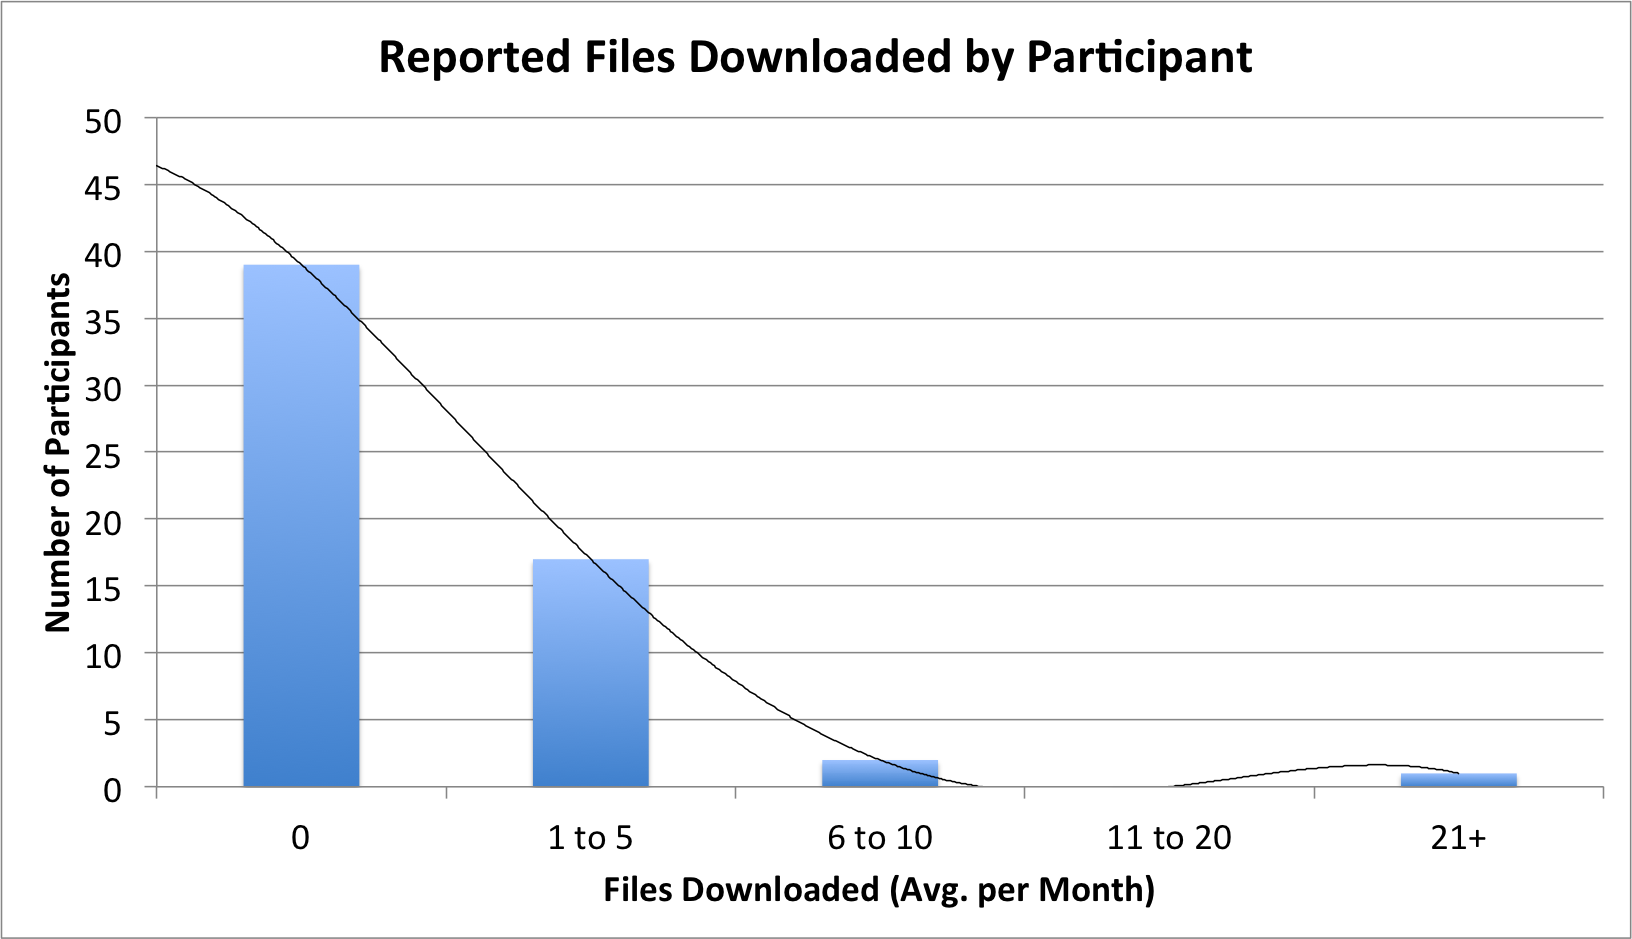
\includegraphics[width=77mm]{Figure3}
	\caption{Bar distribution of reported number of files downloaded via torrenting by the participant.}
	\label{p2p_network}
\end{minipage}
\quad
\centering
\begin{minipage}[b]{0.45\linewidth}
	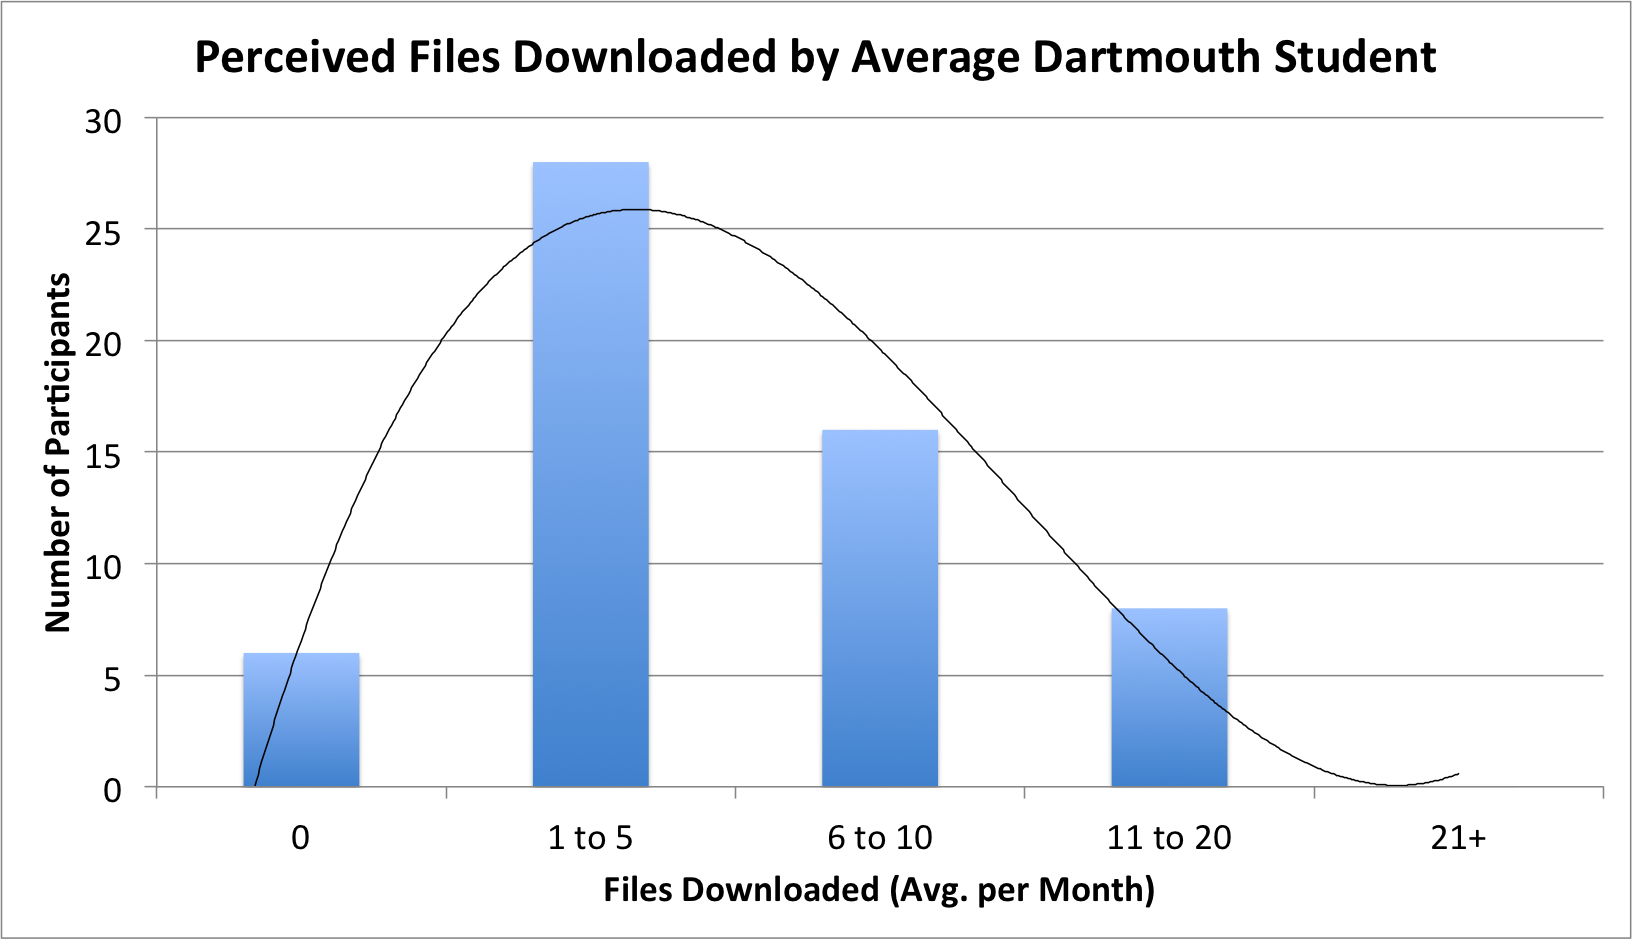
\includegraphics[width=77mm]{Figure4}
	\caption{Bar distribution of perceived number of files downloaded via torrenting by the ``average Dartmouth student.''}
	\label{p2p_network}
\end{minipage}
\end{figure}

With regard to whether participants believed that Dartmouth recorded student torrenting information or whether knowledge of Dartmouth's Copyright Violation Policy affects how often the participant torrents, the results were less conclusive. Of the 130 students asked if Dartmouth records when someone torrents a file, 47 (36.2\%) said Yes; 28 (21.5\%) said No; and 55 (42.3\%) said they were Unsure. Attempting to break down the results further by number of files participants reported downloading or by the number of files that participants perceived that other students download were also inconclusive; more data would need to be collected to determine this result. Regarding whether knowledge of Dartmouth's Copyright Violation Policy affected personal torrenting practices, there was no significant difference (\emph{p}$>$.05) between the number of participants who said Yes (N=63, 48.5\%) and who said No (N=67, 51.5\%). 

\subsection{Dartmouth Network Patterns}
Adam Goldstein, PaloAlto, types of metrics

\subsection{Relationship between Student Perception and Dartmouth Network Data}
Draw some conclusions and relationships between analytics (e.g. perception ? practice)

%%%%%%%%%%%%%%%%%%%%%%%%%%%%%%%%%%%
%%%% ********			  CONCLUSIONS  		******** %%%%%
%%%%%%%%%%%%%%%%%%%%%%%%%%%%%%%%%%%

\section{Conclusion}
Summary, Questions, and Policy Recommendations

%%%%%%%%%%%%%%%%%%%%%%%%%%%%%%%%%%%
%%%% ********			  REFERENCES  		******** %%%%%
%%%%%%%%%%%%%%%%%%%%%%%%%%%%%%%%%%%
\pagebreak
\begin{thebibliography}{9}
\bibitem{BitTorrent} ``BitTorrent: Beginner's Guide.'' \emph{BitTorrent Inc.} Accessed November 4, 2013. Available at http://www.bittorrent.com/help/guides/beginners-guide.
\bibitem{NYTimes} Shannon, Victoria. ``The End User: P2P starts to mature.'' \emph{New York Times}. July 9, 2005. Available at http://www.nytimes.com/2005/07/08/technology/08iht-ptend09.html.
\bibitem{scholl} R�diger Schollmeier, A Definition of Peer-to-Peer Networking for the Classification of Peer-to-Peer Architectures and Applications, Proceedings of the First International Conference on Peer-to-Peer Computing, IEEE (2002).
\bibitem{About} http://compnetworking.about.com/od/p2ppeertopeer/a/p2pintroduction.htm
\bibitem{P2PFileSharewiki} ``Peer-to-peer file sharing.'' \emph{Wikipedia}. Accessed November 4, 2013. Available at http://en.wikipedia.org/wiki/Peer-to-peer\_file\_sharing\#History.
\bibitem{napster} Douglas, Guy. ``Copyright and Peer-To-Peer Music File Sharing: The Napster Case and the Argument Against Legislative Reform.'' \emph{Murdoch University Electronic Journal of Law.} Vol. 11, No. 1 (March 2004). Available at http://www.murdoch.edu.au/elaw/issues/v11n1/douglas111.html.

\bibitem{HTG} http://www.howtogeek.com/141257/htg-explains-how-does-bittorrent-work/
\bibitem{glossary} http://en.wikipedia.org/wiki/Glossary\_of\_BitTorrent\_terms\#Leech

\end{thebibliography}

** statistics on P2P we may want to use: http://www.ipoque.com/sites/default/files/mediafiles/documents/internet-study-2008-2009.pdf

%%%%%%%%%%%%%%%%%%%%%%%%%%%%%%%%%%%
%%%% ********			  APPENDIX	  		******** %%%%%
%%%%%%%%%%%%%%%%%%%%%%%%%%%%%%%%%%%
\newpage
\section*{Appendix A}

\newenvironment{packed_enum}{ % compact list
\begin{itemize}
  \setlength{\itemsep}{1pt}
  \setlength{\parskip}{0pt}
  \setlength{\parsep}{0pt}
}{\end{itemize}}

\newenvironment{question}{ % reduced spacing for questions
  \setlength{\parskip}{0pt}
}

\subsection*{Student Perception Survey}

\begin{enumerate}

\item \begin{question}
\noindent Have you ever downloaded files (music, movies, applications, etc.) via torrenting?
  \begin{packed_enum}
  \item Yes
  \item No
  \end{packed_enum}
\end{question}

\item \begin{question}
\noindent Have you ever downloaded files (music, movies, applications, etc.) via torrenting while at Dartmouth?
  \begin{packed_enum}
  \item Yes
  \item No
  \end{packed_enum}
\end{question}

\item \begin{question}
\noindent On average, how many files do you download via torrenting per month at Dartmouth?
  \begin{packed_enum}
  \item 0
  \item 1-5
  \item 6-10
  \item 11-20
  \item 21+
  \end{packed_enum}
\end{question}

\item \begin{question}
\noindent How many files do you think an average student at Dartmouth downloads via torrenting per month?
  \begin{packed_enum}
  \item 0
  \item 1-5
  \item 6-10
  \item 11-20
  \item 21+
  \end{packed_enum}
\end{question}

\item \begin{question}
\noindent Do you think that Dartmouth records when you or someone else torrents a file?
  \begin{packed_enum}
  \item Yes
  \item No
  \item Unsure
  \end{packed_enum}
\end{question}

\item \begin{question}
\noindent Does your knowledge of Dartmouth's copyright policy affect how often you download files via torrenting?
Dartmouth policy states that, "If your computer begins to consume excessive network resources, Computing Services will investigate your network activities in order to keep the network operating smoothly?.Sanctions [for illegal downloading] may include suspension of network access (meaning loss of e-mail and course web site access) and formal college disciplinary action."
   \begin{packed_enum}
  \item Yes
  \item No
  \end{packed_enum}
\end{question}

\item \noindent Do you have any thoughts on how Dartmouth could reduce student torrenting on campus?

\end{enumerate}

%%%%%%%%%%%%%%%%%%%%%%%%%%%%%%%%%%%
\newpage
\section*{Appendix B}
\subsection*{Email Notice of Unauthorized Use of Copyrighted Property}

Sent: Friday, October 28, 2011 4:01 PM
\\To: ****************
\\Subject: FW: Notice ID: ******** Notice of Unauthorized Use of ************* Corporation Property

Dartmouth College has received a notice claiming that an IP address registered to you has been used to offer for download via the Internet, without permission, a copyrighted work, cited in the complaint below.

Infringement is actionable under federal copyright law and can require the payment of damages of up to 0,000 per violation, as well as carrying the potential for criminal penalties. Respect for intellectual property ownership is a fundamental value in academia. Copyright infringement is also a violation of College policy. Additional information about the College's copyright policy - including peer-to-peer file sharing - can be found online at http://www.dartmouth.edu/copyright/.

By return e-mail, please indicate that (1) you have removed from your computer any programs that may be used to offer copyrighted material via the Internet for download by others without the copyright owner's permission (examples of such programs include BitTorrent and Limewire) and (2) that you will desist from activities that infringe copyright.  If you need assistance in removing file-sharing programs from your computer, the College's Computing Services department would be glad to assist you.  For this purpose, please contact the Student Help Desk or your IT Consultant.

If you fail to respond promptly, the College will block your IP address. The College must take this step in order to avail itself of the legal protection afforded service providers under the Digital Millennium Copyright Act.
Please note, in most cases this notice comes as a result of the uploading or downloading of music, video, audio, movie or television files that, as a functionality of the file-sharing software used for downloading, is available for uploading by Internet requests without your awareness or permission anytime that your computer is turned on. Scans by copyright owners (such as the company that made the complaint in this case) capture both uploading and downloading of these files.

If you believe this notice is in error, or choose to challenge it, please contact me and I will explain the procedure. This procedure entails the filing on your part of a counter-notice asserting your right to the material and your right to distribute it, and satisfying all of the requisite legal formalities. Only after you have filed a proper counter-notice can a request to have your IP address unblocked be granted.

Thank you for your cooperation.  I look forward to hearing from you.

\begin{center}
{- Chief Information Security Officer,
Dartmouth College,
Hanover, NH  03755}
\end{center}

%%%%%%%%%%%%%%%%%%%%%%%%%%%%%%%%%%%
\newpage
\section*{Appendix C}
\subsection*{File Sharing Program Gigabyte Usage\footnote{Provided by Adam Goldstein, Dartmouth College Computing Services.}
}
\textbf{\indent 24 Hour\\\\}
    \begin{tabular}{ | l | l | l | p{5cm} |}
    \hline
    App Sub Category & Application Name & Gigabytes & Percentage \\ \hline
    file-sharing & bittorrent & 177.09 & 70.50  \\ \hline
    file-sharing & dropbox & 44.56 & 17.73  \\ \hline
    file-sharing & ftp & 20.25 & 8.06  \\ \hline
    file-sharing & azureus & 3.42 & 1.36  \\ \hline
    file-sharing & pando & 1.94 & 0.77  \\ \hline
    file-sharing & google-drive-web & 1.53 & 0.61  \\ \hline
    file-sharing & skydrive-base & 1.49 & 0.60  \\ \hline
    file-sharing & boxnet-base & 0.89 & 0.36  \\ \hline
    \end{tabular}

\textbf{7 Day\\\\}
    \begin{tabular}{ | l | l | l | p{5cm} |}
    \hline
    App Sub Category & Application Name & Gigabytes & Percentage \\ \hline
    file-sharing & bittorrent & 1180.17 & 60.10  \\ \hline
    file-sharing & dropbox & 394.77 & 20.10  \\ \hline
    file-sharing & ftp & 313.54 & 15.97  \\ \hline
    file-sharing & pando & 36.40 & 1.85  \\ \hline
    file-sharing & skydrive-base & 12.94 & 0.66  \\ \hline
    file-sharing & boxnet-base & 10.02 & 0.51  \\ \hline
    file-sharing & azureus & 7.69 & 0.39  \\ \hline
    file-sharing & google-drive-web & 7.62 & 0.39  \\ \hline
    \end{tabular}
    
\textbf{30 Day\\\\}
    \begin{tabular}{ | l | l | l | p{5cm} |}
    \hline
    App Sub Category & Application Name & Gigabytes & Percentage \\ \hline
    file-sharing & bittorrent & 4757.79 & 60.89  \\ \hline
    file-sharing & dropbox & 1697.71 & 21.73  \\ \hline
    file-sharing & ftp & 1046.01 & 13.39  \\ \hline
    file-sharing & pando & 137.98 & 1.77  \\ \hline
    file-sharing & azureus & 53.67 & 0.69  \\ \hline
    file-sharing & skydrive-base & 52.94 & 0.68  \\ \hline
    file-sharing & boxnet-base & 33.32 & 0.43  \\ \hline
    file-sharing & google-drive-web & 29.01 & 0.37  \\ \hline
    \end{tabular}

\end{document}
